\section{Evaluation}
\label{sec:evaluation}

The goal of our evaluation is to understand whether the core pieces of the \Grappa
runtime system, namely our tasking system and the global memory/communication
layer work as expected and whether together they are able to efficiently run irregular
applications. We evaluate \Grappa in three basic steps:

\begin{itemize}

\item We present results that show that \Grappa can
    support large amounts of concurrency, sufficient for remote memory
    access and aggregation. The communication layer is able to
    sustain a very high rate of global memory operations. We also show the performance of a
graph kernel that stresses communication and concurrency together.
%\TODO{compare to key-value stores?}

\item We characterize system behavior, including
profiling where execution time goes, and how aggregation affects message size and
rates.

%, and \checkme{the relationship between aggregation and
%    concurrency.}

\item Finally, we show how some more realistic irregular workloads on \Grappa
compare to the Cray XMT and hand-tuned MPI code.

%\comment{
%\TODO{Grappa is well-suited to applications where there is
%    abundant data parallelism but unpredictable or imbalanced data
%    access. BSP is efficient where there is sufficient parallel slack.
%    Although Grappa loses some asynchrony by relying heavily on
%    aggregation, it still provides more flexibility for sections of the
%    computation to proceed more quickly. }
%
%\TODO{how much concurrency is needed on apps. Our basic plot of
%    performance vs workers (with and without aggro?)}
%\TODO{relationship between user-thread-visible latency and aggregate throughput.}
%\TODO{characterization of aggregation message size vs nodes}
%\TODO{show our scalability plots; if they don't scale, show
%    specifically why. It is okay if its because aggregation stops
%    working after a point if we can discuss future scalability.
%    Perhaps reference ``MPI on millions of cores'' type work}
%}
\end{itemize}

\subsection{Basic \Grappa Performance}
\label{eval:basic}

\paragraph{User-level context switching.}

Fast context switching is at the heart of \Grappa's
latency tolerance abilities. We assess context switch overheads using a simple
microbenchmark that runs a configurable number of workers on a single core, where each worker 
increments values in a large array. 

\begin{figure}[ht]
    \begin{center}
      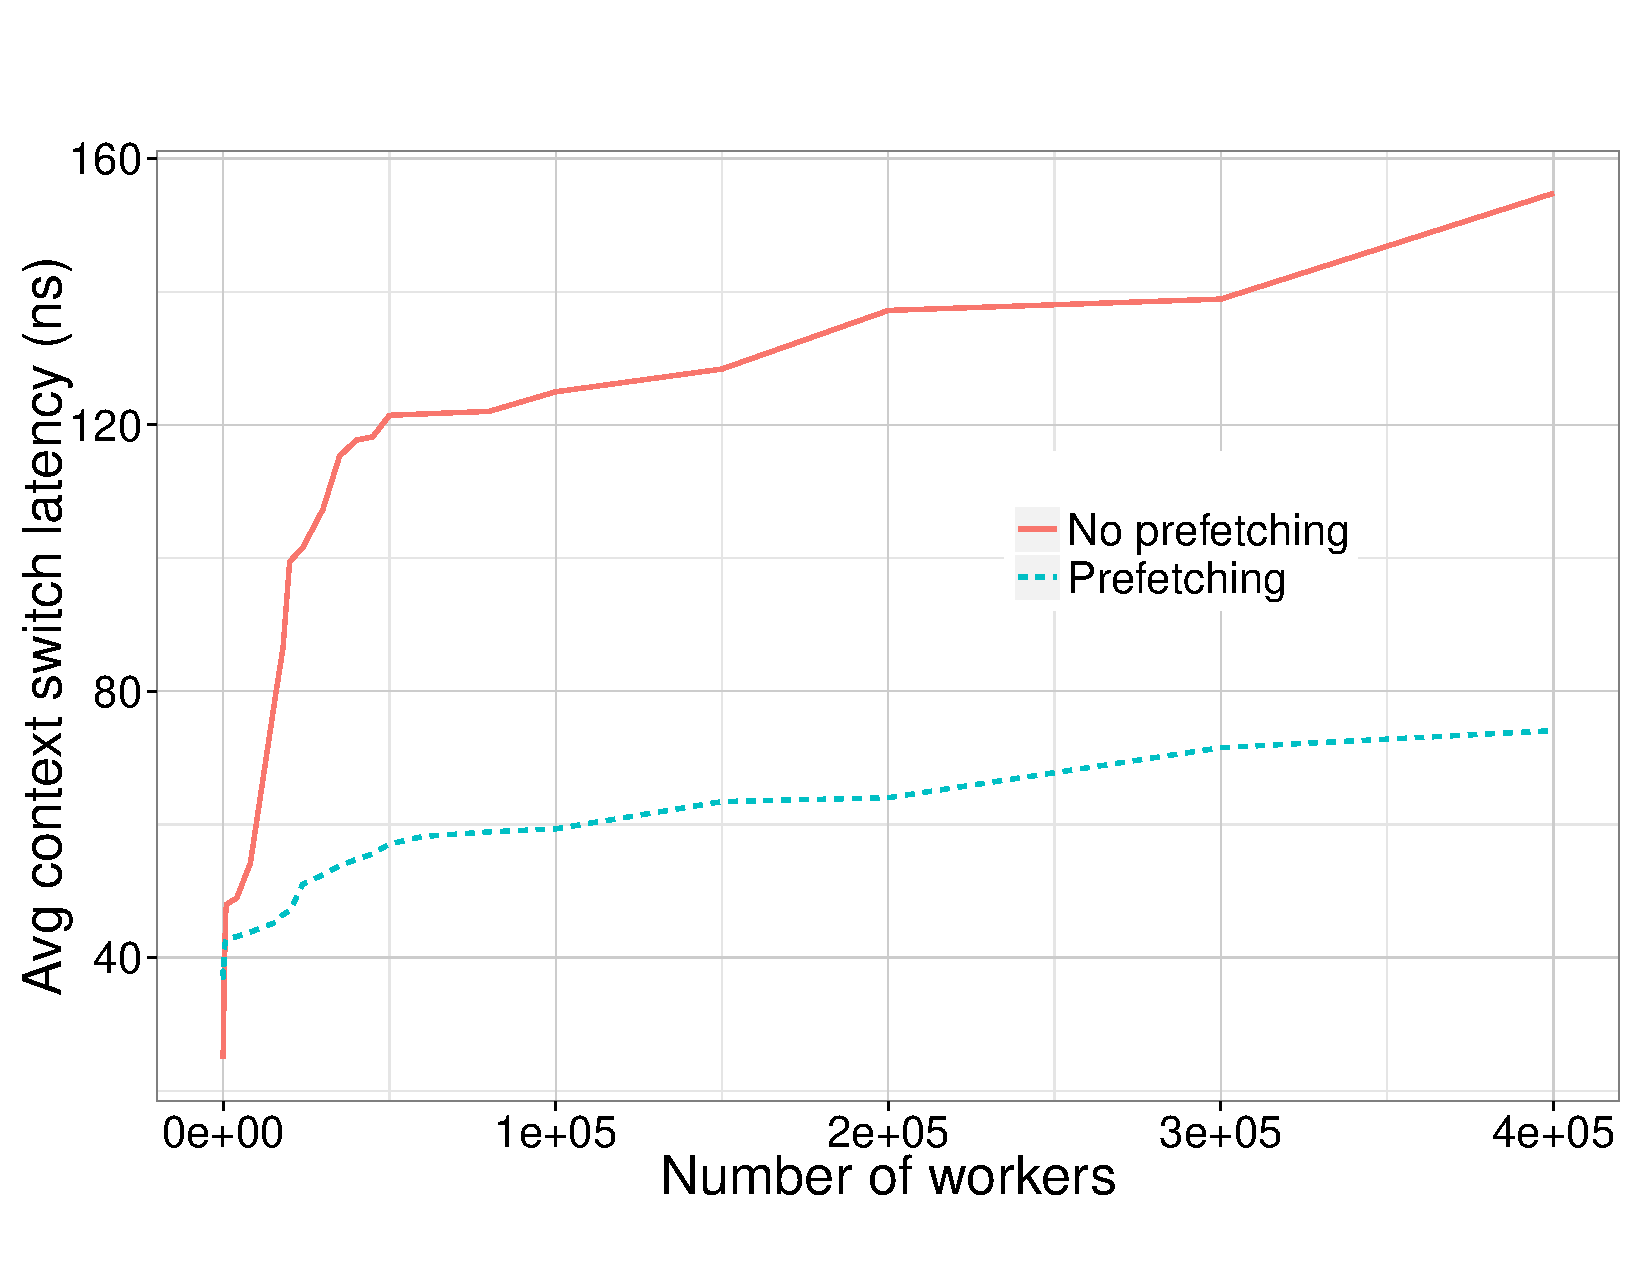
\includegraphics[width=0.5\textwidth]{figs/context_switch_time.pdf}
    \end{center}
    \caption{Average context switch time with and without prefetching.}
    \label{fig:context-switch-exp}
\end{figure}

Figure~\ref{fig:context-switch-exp} shows the average context switch
time as the number of workers grow. At our standard operating point
($\approx$1K workers), context switch time is on the order of
50ns. As we add workers, the time increases slowly, but levels off:
we also ran with 500,000 workers (10~times what is shown in the
figure) and found that context switch time was around 75ns. In
comparison, for the same yield test using kernel-level Pthreads on a
single core, the switch time is 450ns for a few threads and 800ns for
1000--32000 threads.

If we calculate aggregate context switch \emph{rate\/} of all
cores in a node, we find that with prefetching, \Grappa context
switching is
limited \emph{not\/} by memory latency, as normally assumed, but rather memory bandwidth.
Specifically, we empirically found that 4~cache lines (1~for worker
struct and 3 for stack data) was sufficient to avoid cache misses in
the microbenchmark. Every context switch then requires 8~cache-line transfers. The off-chip
bandwidth of a single socket in our system is 270M cache lines per
second~\cite{porterfield:bw,Nelson:hotpar11}. This implies that, in the limit,
we can sustain at most 34M context switches per second per socket (a context-switch time of 29ns).

In summary, our tasking layer is able to efficiently sustain very high
concurrency and, as we will show later, the amount of concurrency sustained is
sufficient for the latencies \Grappa needs to hide.

\paragraph{Global memory and communication.} We measure the performance of
\Grappa's global memory and communication layers using a faithful
implementation of the giga updates per second (GUPs) benchmark, which
measures cluster-wide random access bandwidth.  Read-modify-write
updates are dispatched at random to a global large array. This benchmark
stresses the communication layer of \Grappa separately from the
scheduler, because only a single worker is used per system node.
Figure~\ref{fig:grappa-gups} shows that \Grappa is able to sustain
well over a billion updates per second with 64~nodes. Note also that
when aggregation is turned off, the update rate is nearly
flat. Clearly aggregation is instrumental for good communication
performance.

This compares very favorably to published results~\cite{gups} for other
high-end HPC systems. Though the actual computation done by GUPS is not 
useful, irregular, data-intensive applications typically must be able to
sustain a high rate of random accesses in order to, for example, visit and
mark vertices during a graph traversal. High random access rate in a
distributed setting has been a long-standing challenge in HPC.

\begin{figure}[ht]
    \begin{center}
      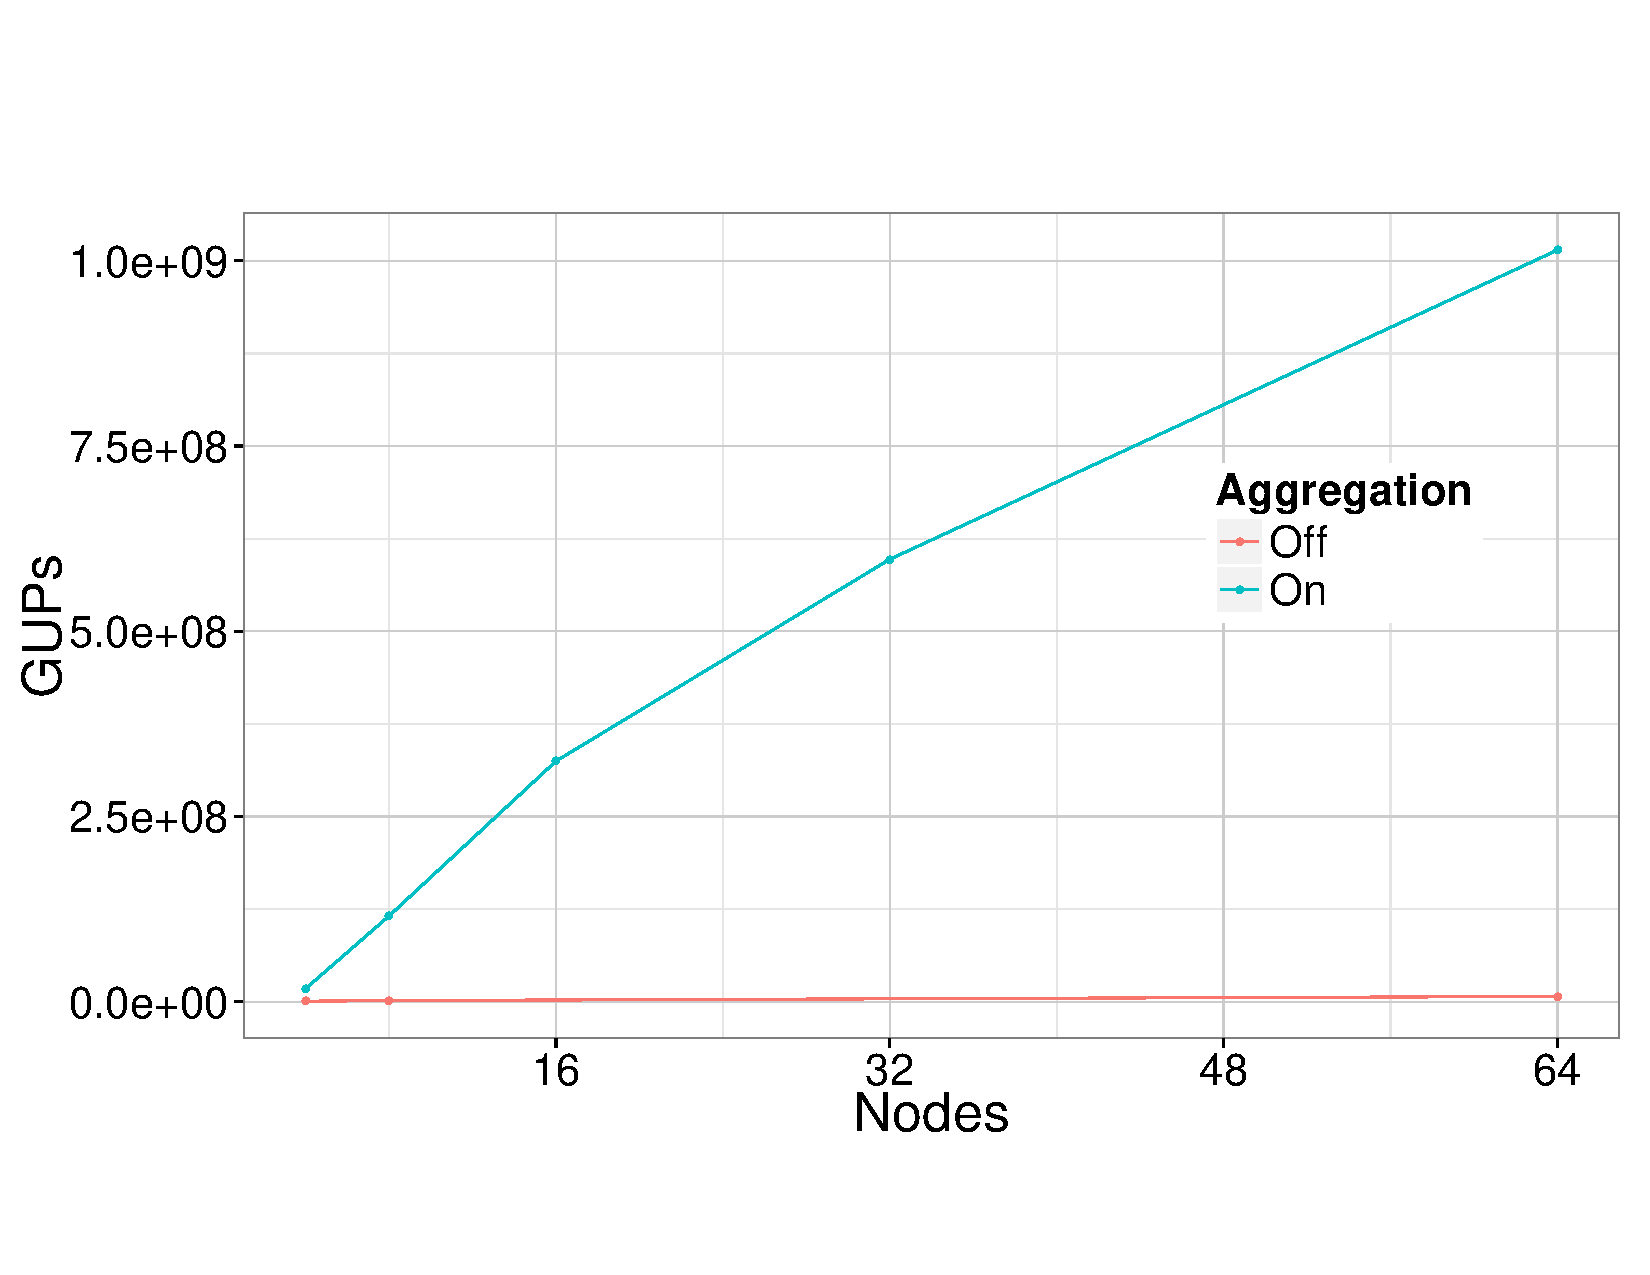
\includegraphics[width=0.5\textwidth]{figs/gups.pdf}
    \end{center}
    \caption{GUPS (giga updates per second) for \Grappa as the number of nodes grows with and without message aggregation.}
    \label{fig:grappa-gups}
\end{figure}

%\TODO{go into more detail about what Grappa is doing when executing
%    GUPs. Specifically note what the rate per core is, what the
%    aggregation and deaggregation rates are. Show on the plot the
%    message size distribution (some box plot)}

\paragraph{Putting it all together with Unbalanced Tree Search in memory
(UTS).} 
Figure~\ref{fig:grappa-uts} shows the overall performance of \Grappa running
UTS. This experiment demonstrates that \Grappa's context
switching and communication layers can be used together, while
balancing workload, to run an irregular application efficiently. 

Visiting vertices in the distributed tree requires mostly remote
accesses, and because each vertex in the tree must be visited before
it can be expanded, blocking remote reads are required. In this case,
we are forced to context switch to tolerate the remote access and
continue aggregating.

We look at two classes of trees, T1 and T3, from
the original benchmark. T1 trees are very shallow and wide (i.e., significant
parallel slack \cite{Valiant:1990}), while T3 trees are very deep (i.e., little parallel slack).
Given that access to each vertex is a random access, the critical path to search
T3 trees is very long, hence the low performance and scalability. On such
trees, we do not expect there to be sufficient concurrency for any system,
including \Grappa, to achieve high throughput -- at the 16-node data point,
the average active tasks per core over the search is 775 for T1 and
only 13 for T3. Given the lack of parallelism, scaling up only serves
to reduce throughput by distributing the tree to more machines.
On the other hand, \Grappa performs and scales very well for T1
trees.

We compared this to a in-memory modification of the UPC implementation
of UTS \cite{UTS}, where each core hosts a UPC ``THREAD''. Berkeley
UPC (BUPC) is built upon GASNet, like Grappa, but it uses RDMA transfers directly
and the compiler overlaps remote communication when possible. We expect BUPC to
perform similarly on the T3 tree, where there is little parallelism to
overlap communication and computation, and no better than T3 on T1,
given the inability to overlap vertices on each core without
multithreading (a multithreaded variant of UPC has been evaluated in
\cite{HotSLAW}). Our experiments confirm that BUPC achieves the lower throughput of
Grappa on T3 for \emph{both} the T1 and T3 trees. 

\begin{figure}[ht]
    \begin{center}
      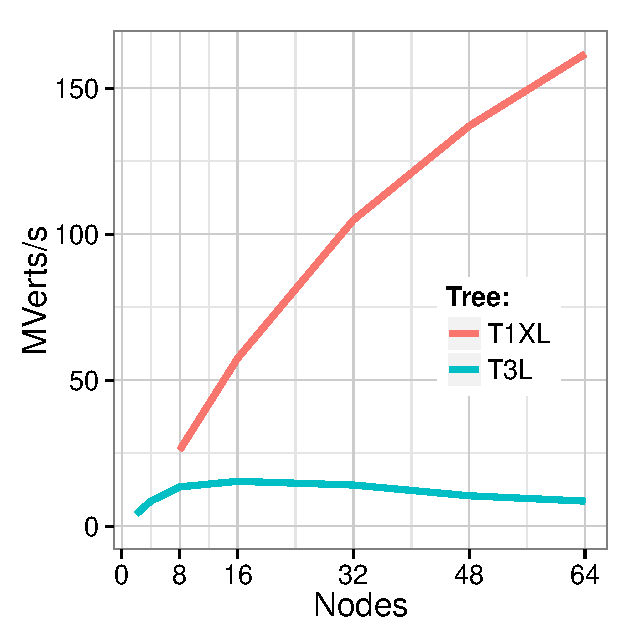
\includegraphics[width=0.36\textwidth]{results/plot_scaling_uts.pdf}
    \end{center}
    \caption{Vertices per second in UTS on \Grappa as the number of nodes grows.}
    %\TODO{modify discussion inline to match new plot}}
    \label{fig:grappa-uts}
\end{figure}

\subsection{Comparing \Grappa to Other Systems}
\label{eval:mainperf}

In order to put \Grappa's performance into a general context, we compare it
with XMT running BFS, PageRank, IntSort, GUPS and UTS. Since XMT is a
different hardware platform, we also compare \Grappa with optimized MPI
versions of BFS and GUPS running on the same hardware. Finally, we also
compare it with UTS written for UPC. We run all experiments with 64 nodes and 16 cores per node.

% \begin{figure}[ht]
%     \begin{center}
%       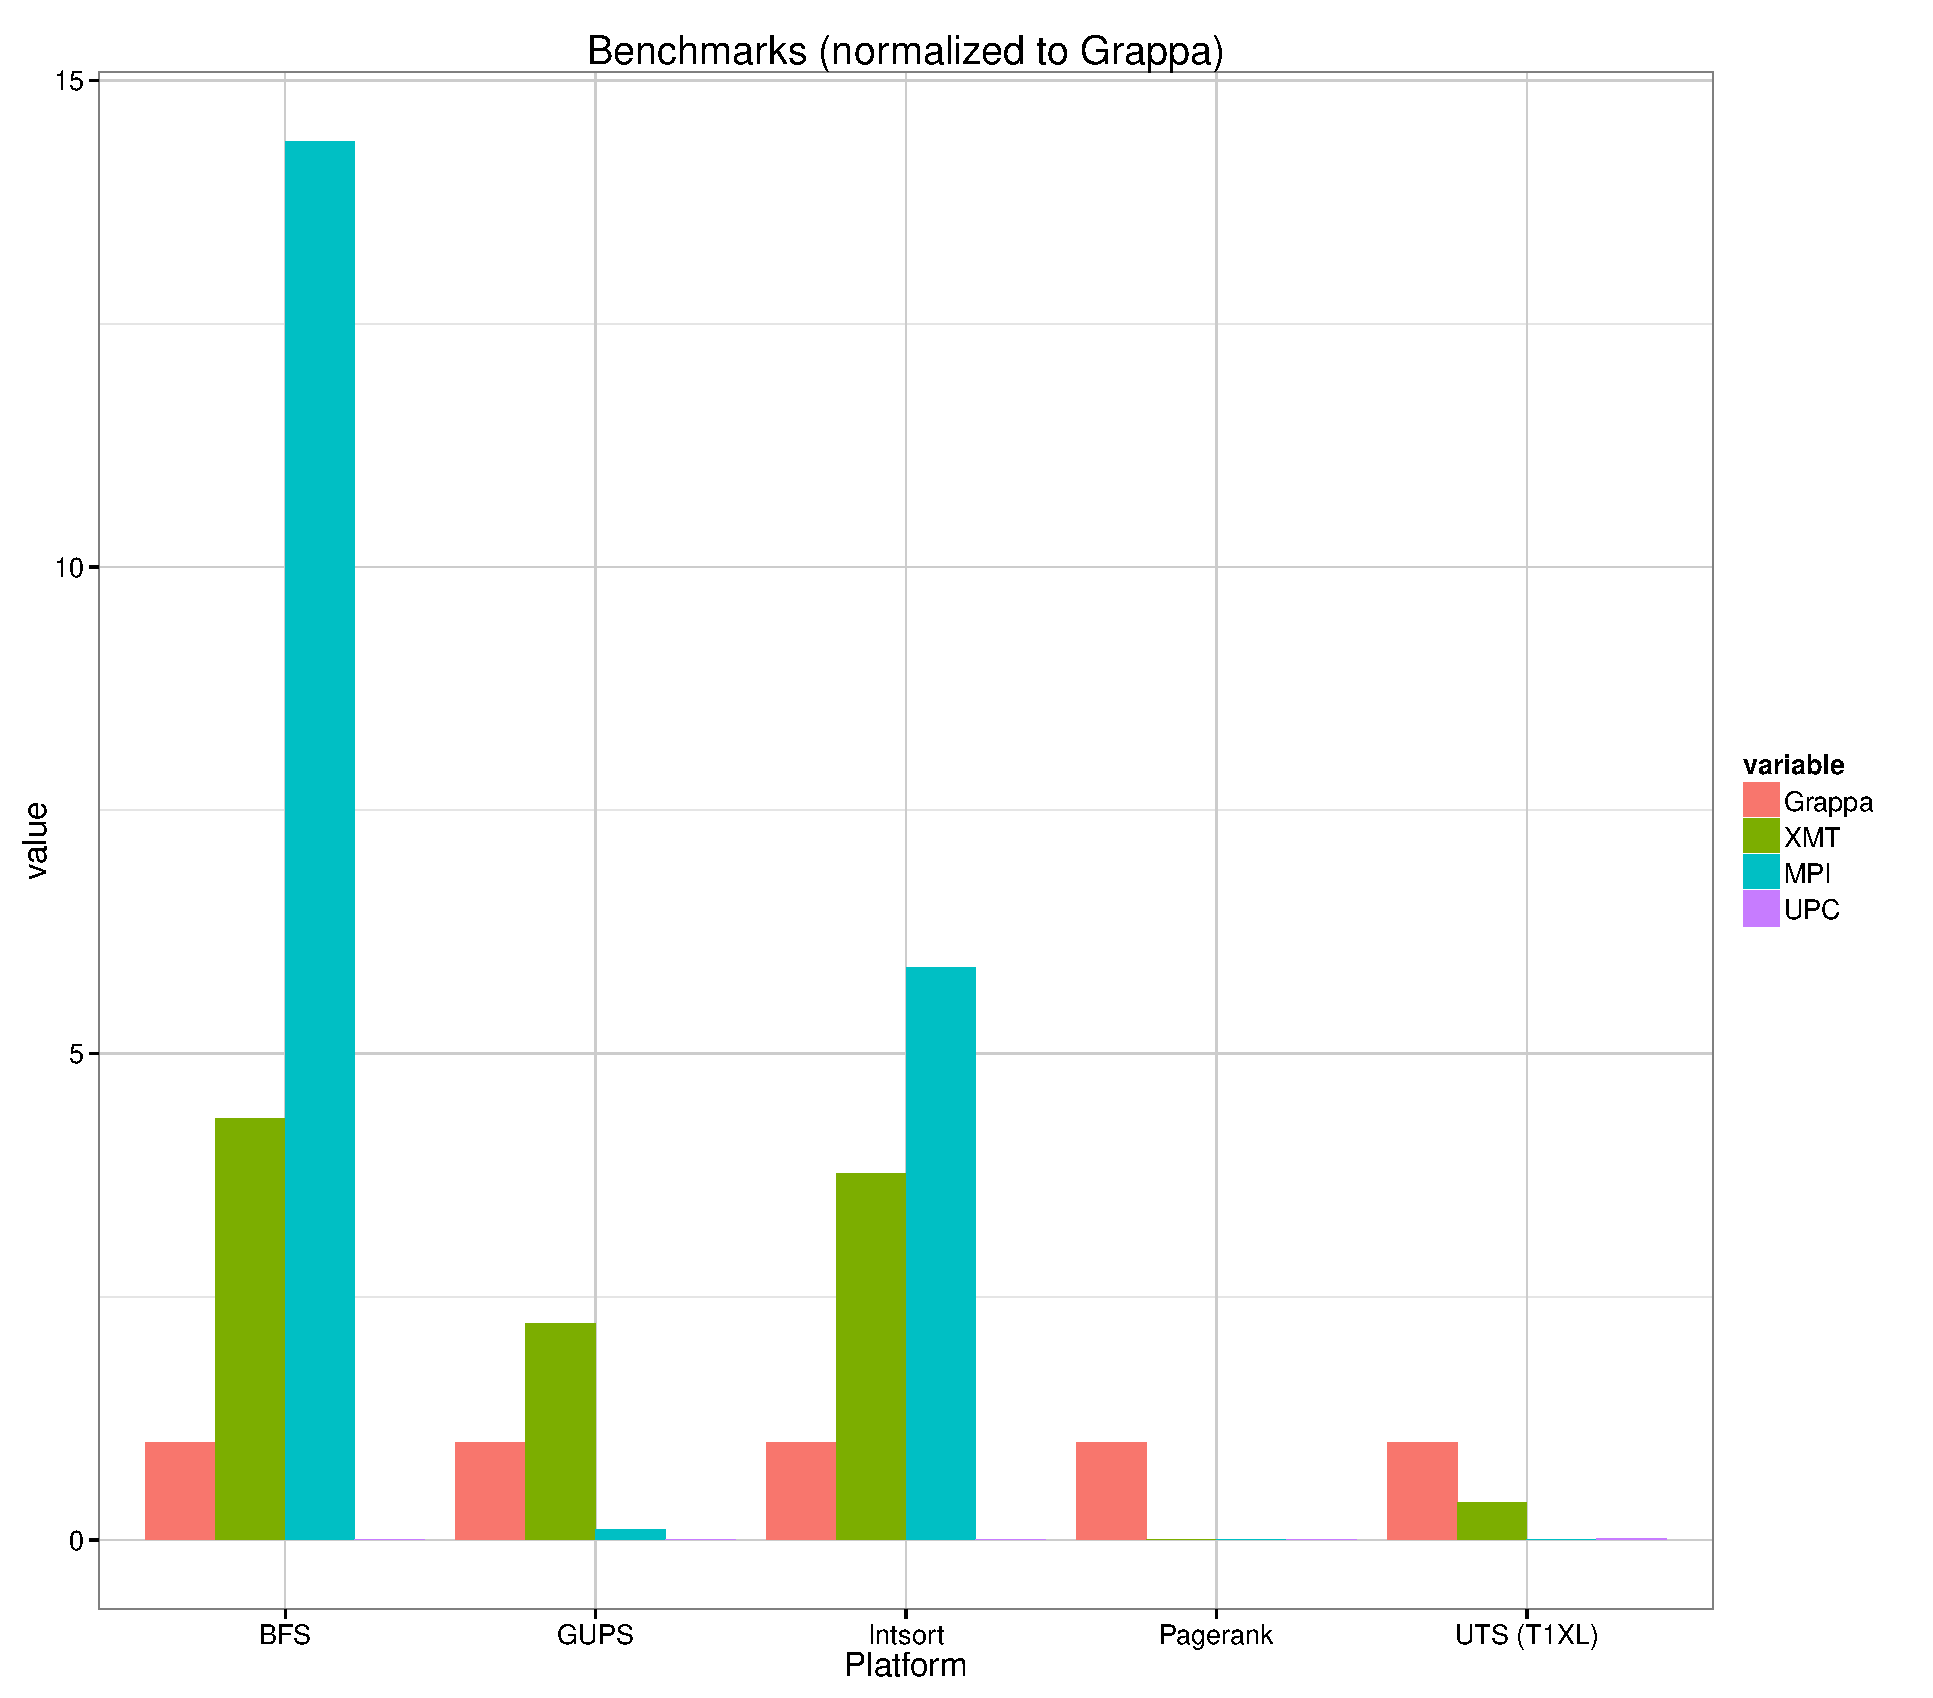
\includegraphics[width=0.5\textwidth]{results/benchmarks.pdf}
%     \end{center}
%     \caption{Comparing \Grappa with XMT, hand-tuned MPI and UPC.}
%     \label{fig:grappa-comparisons}
% \end{figure}

\begin{table}[htb]
\begin{center}
\begin{tabular}{l|c|c|c}
         & \Grappa & XMT   & MPI   \\ \hline
GUPS     & 1       & 2.23  & 0.11 \\ 
BFS      & 1       & 1.63  & 3.52 \\ 
IntSort  & 1       & 3.59  & 5.36 \\
UTS (T1) & 1       & 0.38  & --   \\  % 0.09 for UPC
Pagerank & 1       & 4.35  & 4.87 \\ 
\end{tabular}
\end{center}
\caption{Comparing \Grappa with XMT and optimized MPI. Numbers are presented as throughput on 64 nodes normalized to \Grappa.}
\label{tab:grappa-comparisons}
\end{table}

Table~\ref{tab:grappa-comparisons} shows the results. \Grappa is able
to provide performance approaching and sometimes exceeding that of the
other systems. This data shows that, while \Grappa is good at the
operations for which it was designed, there is a cost to providing
\Grappa's generality. In general, the benchmarks whose MPI
implementations are faster than \Grappa include a implementation of a
subset of \Grappa's functionality specialized for their particular
problem. We now discuss each benchmark in more detail.

\paragraph{UTS.}
It is perhaps not surprising that the XMT is faster than
\Grappa on many of the benchmarks; after all, the XMT is custom
hardware optimized for irregular applications. The XMT can
context-switch every cycle, while \Grappa takes $~$50 ns. The XMT can
complete 100 million random-access remote reads per second per node in
hardware, while \Grappa must spend many instructions managing and
aggregating each of these reads in software.

What is more surprising is that \Grappa is able to exceed the XMT's
performance on UTS. This is a demonstration of the inflexibility of
custom hardware. Recall that the UTS benchmark searches an unbalanced
tree and spawns a data-dependent number of child tasks at each
vertex. The XMT's spawn/join semantics, whose implementation is spread
across the hardware, OS, and runtime, require a task visiting a vertex
to block until all its child tasks have completed, even though the
benchmark does not require those tasks to have completed until the end
of the tree search. Furthermore, each new task is immediately made
available to all other processors in the system, even though it is
likely that processor that spawned a task will end up executing it.

Since \Grappa's tasks are implemented entirely in software, it is easy
to support arbitrary synchronization semantics. \Grappa allows both
XMT-like per-vertex task joins as well as whole-problem joins that are
a better fit for UTS. Furthermore, \Grappa's work-stealing distributed
task queue and recursive loop decomposition encourage locality in task
execution, so that the system is optimized for the common case of a
processor executing a task it spawned.

We also compare with an UPC UTS implementation, which is nearly 10$\times$
\emph{slower} than \Grappa. Our UPC version supports work-stealing but has
limited ability to overlap communication with computation. Also, it
employs heavyweight synchronization operations when stealing. \Grappa
benefits from its lightweight context switching and support for fine-grained
synchronization.

\paragraph{BFS.}
The \Grappa and MPI BFS implementations are quite similar. They both
use the same graph representation, and they both depend on aggregation
for performance. The difference is that the BFS' aggregation is
integrated with the traversal code and specialized for the problem:
since the only messages required are edge traversals, the aggregation
buffers store only pairs of 8-byte vertex IDs.  In contrast, \Grappa
pays execution and space overhead in order to support aggregation of
arbitrary messages; the messages \Grappa aggregates include the two
8-byte vertex IDs along with 8 bytes of deserialization information as
well as 8 bytes of synchronization information. Furthermore, the MPI
implementation writes the edge information directly into the
aggregation buffer while \Grappa executes additional code to serialize
and deserialize the messages.

\paragraph{GUPS.}
The MPI GUPS implementation includes an implementation of aggregation,
but it is not optimized to work when the aggregated data exceeds
cache, and it has limited support for concurrent communication with
multiple destinations. \Grappa benefits from being optimized for both
of these cases.

\paragraph{Pagerank.}
The MPI Pagerank implementation is built on top of the
highly-optimized sparse matrix support in the Trilinos~\cite{trilinos}
library. In contrast, the \Grappa implementation is a straightforward nested
loop.

\paragraph{IntSort.}
Both MPI and \Grappa IntSort implement a bucket sort. For \Grappa,
distributing keys into buckets accounts for the bulk of the execution
time; \Grappa does this using asynchronous delegate operations to
write the keys directly to their final destination. The MPI
implementation, on the other hand, first does a local sort of the keys
on each core, and then uses an \texttt{MPI\_Alltoallv()} collective
operation to move all the keys to their destination nodes in
bulk. This is essentially specialized aggregation combined with
collective communication. When we measure the time spent in this
region of both benchmarks, we find that the the sort and
\texttt{MPI\_Alltoallv()} are $~5\times$ faster than the \Grappa
version using generic aggregation and point-to-point communication. An
interesting future direction would be to extend \Grappa to support
aggregation via collective operations.


\paragraph{Summary.}

Overall, \Grappa provides a general programming model at a moderate
performance cost. While \Grappa's core functionality performs well,
applications can specialize similar functionality for their problems
and obtain better performance than \Grappa on the same hardware. This
is, however, not the end of the story for \Grappa's performance;
\Grappa is a young library and, as discussed in the next section, is
limited by its implementation rather than the hardware on which it
runs. We believe there are opportunities for optimization that will
improve its performance.

\subsection{Characterization}

\begin{table}[htb]
\small
\begin{center}
\setlength{\tabcolsep}{1pt}
\begin{tabular}{l|c|c|c|c|c}
% remember: bfs time is mean_time * nbfs
                               &   GUPS            &   BFS   & IntSort & UTS & Pagerank \\ \hline
App. message rate/core (K/s)  & 984            &  983   &      &     \\
%Application message bytes     & 31.8 $\pm$ 1.2    & \\
Avg. App. message bytes & 31.8              & 33.9    &      & \\
Network BW per node (MB/s)    & 478           & 511 &    &      \\
%Network message bytes         & 23.2K $\pm$ 12.4K & \\ \hline
Avg. Network message bytes     & 23.2K             & 4.3K    & &    \\ \hline
Avg. active tasks/core         & 0.9               & 58.2    &  &  \\
Max. active tasks/core         & 1                 & 128     &  &   \\
Avg. ready queue length/core   & 2.3               & 6.1     &  &    \\
Avg. Ctx switch rate/core (K/s) & 34.2           & 539  &     &  \\ 
Steal count                    & 0                 & 0       &  &     \\
\end{tabular}
\end{center}
\caption{Internal runtime metrics, for 64-node, 16-core-per-node benchmark runs}
\label{tab:grappa-metrics}
\end{table}

\paragraph{Runtime metrics}
Table~\ref{tab:grappa-metrics} show a number of internal runtime
metrics collected while executing the benchmarks from the previous
section. These are per-core averages computed over all 1024 cores of
the 64-node, 16-core-per-node jobs.

The first group of four metrics relate to the communication
layer. Application messages refer to those issued by the user code;
network message refer to the aggregated packets sent over the wire. The
data show that most application messages are only a handful of bytes,
but our aggregator is able to turn them into packets of many kilobytes.

The next group of five metrics relate to the scheduler. We show the
average and maximum number of concurrently-executing tasks, along with
the average length of the ready queue and the average context switch
rate.  The last line shows the number of time a core stole work from
another core. Only UTS depends on work-stealing for performance; the
other applications exploit locality by binding tasks to specific cores
Nevertheless, even in UTS, which depends on work-stealing for
performance, steals are an infrequent occurrence and account for a
small fraction of the execution time.



\begin{figure}[ht]
    \begin{center}
      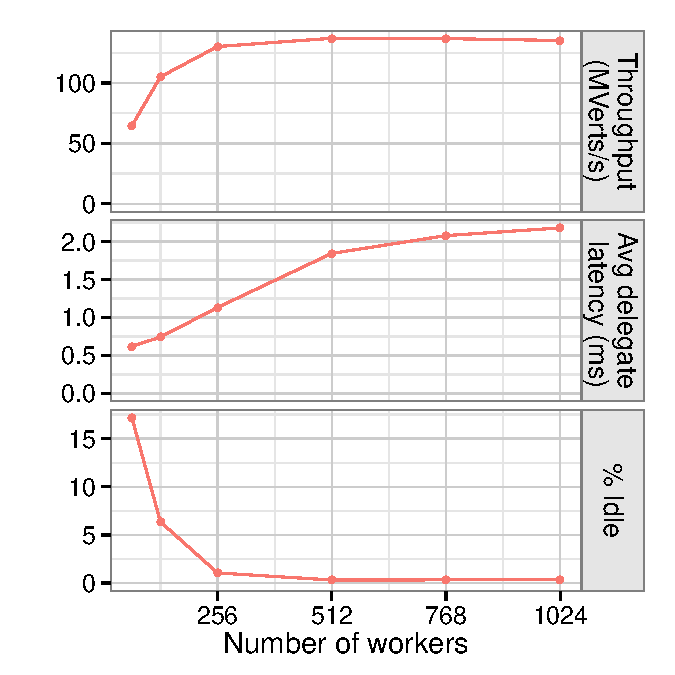
\includegraphics[height=0.5\textwidth, angle=90]{results/plot_concurrency.pdf}
    \end{center}
    \vspace*{-0.25in}
    \caption{Throughput, request latency, and idleness as number of concurrent workers is varied}
    \label{fig:grappa-concurrency}
\end{figure}

\paragraph{How much concurrency does \Grappa require? How much latency does it add?}
\Grappa depends on concurrency to cover the latency of aggregation and
remote communication. How much is required for good performance?

Figure~\ref{fig:grappa-concurrency} shows a 48-node, 16-core-per-node
run of UTS, varying the number of concurrently executing tasks on each
core. The top pane shows the overall throughput of the tree search.
The middle pane shows average blocking delegate operation latency in
microseconds. The bottom pane shows idle time; that is, the fraction
of the time the scheduler could not find a ready task to run.

We can observe three things from this figure. First, above 512
concurrently executing tasks per core, idle time is practically zero:
these tasks generate requests fast enough to cover the latency of
aggregation and communication. This matches the results seen in the
throughput plot; throughput peaks at 512 workers and gradually
decreases after that due to the overhead of unnecessary context
switches. Finally, we see that with 512 workers, the average
per-request latency is $~$1.8ms.

\paragraph{Does \Grappa scale?}


\begin{figure*}[ht]
    \begin{center}
      \subfloat[BFS]{ 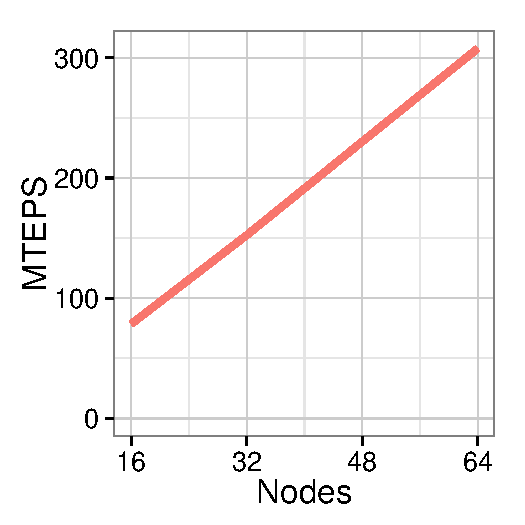
\includegraphics[height=0.25\textwidth]{results/plot_scaling_bfs.pdf} }\qquad
      \subfloat[IntSort]{ 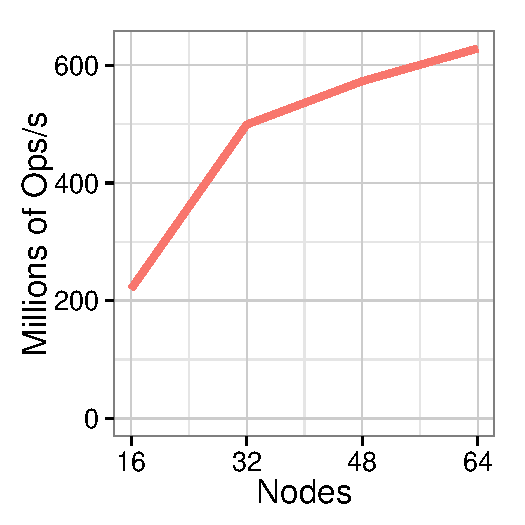
\includegraphics[height=0.25\textwidth]{results/plot_scaling_intsort.pdf} }\qquad
      \subfloat[Pagerank]{ 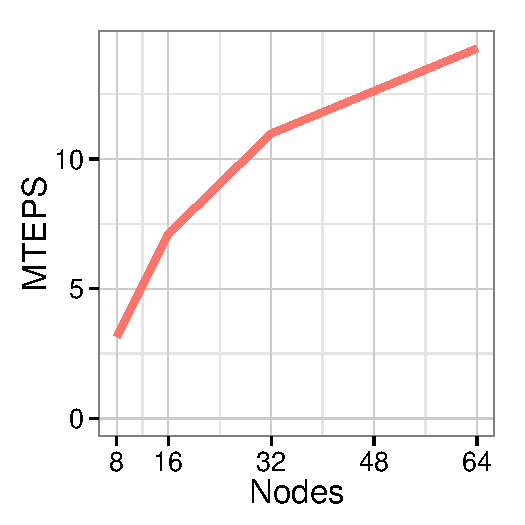
\includegraphics[height=0.25\textwidth]{results/plot_scaling_pagerank.pdf} }\qquad
    \end{center}
    \caption{Scaling for BFS, IntSort, and Pagerank. Refer to Figure~\ref{fig:grappa-gups} for GUPS scaling and Figure~\ref{fig:grappa-uts} for UTS scaling}
    \label{fig:grappa-scaling}
\end{figure*}

Figures~\ref{fig:grappa-scaling}, \ref{fig:grappa-gups}, and
\ref{fig:grappa-uts} show scaling out to 64 nodes. \Grappa scales best
on BFS and worst on IntSort, but is in general able to make use of
more nodes. Unfortunately memory limitations in our current network
library keep us from exploring scaling beyond 64 nodes; this will be
addressed in future work.

In the limit, aggregation does not scale: the time it takes to
aggregate enough random requests to build a buffer of reasonable size
scales with the size of the cluster. However, we believe our current
approach will work for clusters with hundreds of nodes. In the future,
we will explore hierarchical, collective techniques to aggregate
requests from multiple nodes as well; we believe this can apply to
clusters with thousands of nodes.

\paragraph{What limits \Grappa's performance?}
The most common operation in \Grappa is sending a message. Three key
operations occur in a message's lifetime: creating and enqueuing a
message, serializing a message in the aggregator, and deserializing a
message at the destination. We benchmarked each of these steps
individually to shed light on the mechanism.

Minimum-sized messages can be created and enqueued at a rate of 16M/s,
serialized into an aggregation buffer at 32M/s, and deserialized from
an aggregation buffer at 210M/s.  Together, these rates limit us to
$~$10M/s per core in the best case. In a blocking application, the
context switch costs (50ns, or 20M/s) bring this maximum down to
7M/s. In practice, \Grappa does not achieve this maximum; the current
aggregator design communicates inefficiently between cores within a
node, limiting our message rate to to $~$1M/s per core with messages
of common sizes. Future work will reduce this cost.  







